\hypertarget{green-it-les-petits-gestes}{%
\section{Green IT : Les petits
gestes}\label{green-it-les-petits-gestes}}

Ce document est un complément de la présentation
\href{https://prezi.com/view/qpvCT5y3PdddpkdkU7Z4}{Green IT: les vrais
petits gestes}.\\
Si des erreurs ou des fautes sont présentes, n'hésitez pas à faire une
PR.

\begin{itemize}
\tightlist
\item
  \protect\hyperlink{green-it--les-petits-gestes}{Green IT : Les petits
  gestes}

  \begin{itemize}
  \tightlist
  \item
    \protect\hyperlink{les-bonnes-nouvelles}{Les bonnes nouvelles}

    \begin{itemize}
    \tightlist
    \item
      \protect\hyperlink{introduction}{Introduction}
    \item
      \protect\hyperlink{co2-je-te-hais-mais-comment-sen-passer}{CO2 je
      te hais, mais comment s'en passer}
    \item
      \protect\hyperlink{chauffe-marcel}{Chauffe Marcel}
    \item
      \protect\hyperlink{2050}{2050}
    \end{itemize}
  \item
    \protect\hyperlink{le-green-it-notre-sauveur}{Le green IT notre
    sauveur}

    \begin{itemize}
    \tightlist
    \item
      \protect\hyperlink{les-origines-10}{Les origines \emph{{[}10{]}}}
    \item
      \protect\hyperlink{en-pratique}{En pratique}
    \item
      \protect\hyperlink{et-lhumain}{Et l'humain}
    \end{itemize}
  \item
    \protect\hyperlink{vous}{Vous}

    \begin{itemize}
    \tightlist
    \item
      \protect\hyperlink{se-situer}{Se situer}

      \begin{itemize}
      \tightlist
      \item
        \protect\hyperlink{tableau-impact-fabriction}{Tableau impact
        fabriction}
      \end{itemize}
    \item
      \protect\hyperlink{des-bonnes-intentions-mais}{Des bonnes
      intentions mais}
    \end{itemize}
  \item
    \protect\hyperlink{comment-ruxe9duire-son-empreinte-individuelle-}{Comment
    réduire son empreinte individuelle ?}
  \item
    \protect\hyperlink{les-premiers-gestes}{Les premiers gestes}
  \item
    \protect\hyperlink{les-gestes-demandant-un-changement-de-mentalituxe9}{Les
    gestes demandant un changement de mentalité}
  \item
    \protect\hyperlink{investir-pour-duxe9carboner}{Investir pour
    décarboner}

    \begin{itemize}
    \tightlist
    \item
      \protect\hyperlink{le-logement}{Le logement}
    \item
      \protect\hyperlink{les-vuxe9hicules}{Les véhicules}
    \end{itemize}
  \item
    \protect\hyperlink{la-biodiversituxe9}{La biodiversité}

    \begin{itemize}
    \tightlist
    \item
      \protect\hyperlink{quelques-chiffres}{Quelques chiffres}
    \item
      \protect\hyperlink{dans-mon-jardin}{Dans mon jardin}
    \item
      \protect\hyperlink{dans-ma-maison-et-en-vacances}{Dans ma maison
      et en vacances}
    \end{itemize}
  \end{itemize}
\end{itemize}

Licence : \href{LICENSE.txt}{CREATIVE COMMONS BY}\\

\includegraphics{img/CC-BY_icon.svg.png}

\hypertarget{les-bonnes-nouvelles}{%
\subsection{Les bonnes nouvelles}\label{les-bonnes-nouvelles}}

\hypertarget{introduction}{%
\subsubsection{Introduction}\label{introduction}}

\emph{Dormez tranquille jusqu'en 2100} ce livre écrit par Jean-Marc
Jancovici (je ne l'ai pas encore lu) est une bonne accroche pour
commencer cette présentation.

On parle souvent de notre empreinte carbone, de la fin du monde, de la
décroissance, des catastrophes naturelles. Certaines personnes, très
souvent politisées, vont accuser le modèle néo-capitaliste occidental et
vous faire passer pour des personnes ignorantes, non éclairées. Même si
l'on ne peut nier que notre mode de vie est en grande partie responsable
de notre empreinte environnementalle, il ne faut pas tomber dans
l'écueil du :

\begin{quote}
``Ce n'est pas de ma faute ! Mais celle de la société !'' ou bien ``Je
suis la cause de tous les désastres à venir.''
\end{quote}

Le monde n'est ni tout blanc, ni tout noir mais fait d'une multitude de
nuances de gris.

\hypertarget{co2-je-te-hais-mais-comment-sen-passer}{%
\subsubsection{CO2 je te hais, mais comment s'en
passer}\label{co2-je-te-hais-mais-comment-sen-passer}}

Première bonne nouvelle:

\begin{itemize}
\tightlist
\item
  dans une Europe à 27 pays, La France se situe à la 11\^{}ème place des
  pays les moins émetteur de CO2 (\(10,1 tCO_{2eq}\))
  \emph{\href{https://bonpote.com/les-infographies-bon-pote/}{1}}.
\end{itemize}

\begin{quote}
L'équivalent dioxyde de carbone (équivalent CO2) est une mesure métrique
utilisée pour comparer les émissions de divers gaz à effet de serre sur
la base de leur potentiel de réchauffement global (PRG) , en
convertissant les quantités des divers gaz émis en la quantité
équivalente de dioxyde de carbone ayant le même potentiel de
réchauffement planétaire.
\end{quote}

Si l'on se compare à nos voisins ayant un développement économique et
industriel équivalent
\emph{\href{https://bonpote.com/les-infographies-bon-pote/}{1}} :

\begin{itemize}
\tightlist
\item
  Nous émettons un peu plus de CO2 que l'Italie (\(9,9 tCO_{2eq}\)),
\item
  Nous émettons beaucoup moins de CO2 que l'Allemagne
  (\(14,6 tCO_{2eq}\)),
\item
  Nous émettons beaucoup plus de CO2 que l'Espagne (\(8,8 tCO_{2eq}\)).
\end{itemize}

Au niveau mondial, l'UE fait office d'exemple. Depuis 2008, que ce soit
en production et importation nette de \(CO_2\), les émissions ont baissé
\emph{\href{https://www.statistiques.developpement-durable.gouv.fr/edition-numerique/chiffres-cles-du-climat/5-empreinte-carbone-et-emissions-territoriales}{2}}.
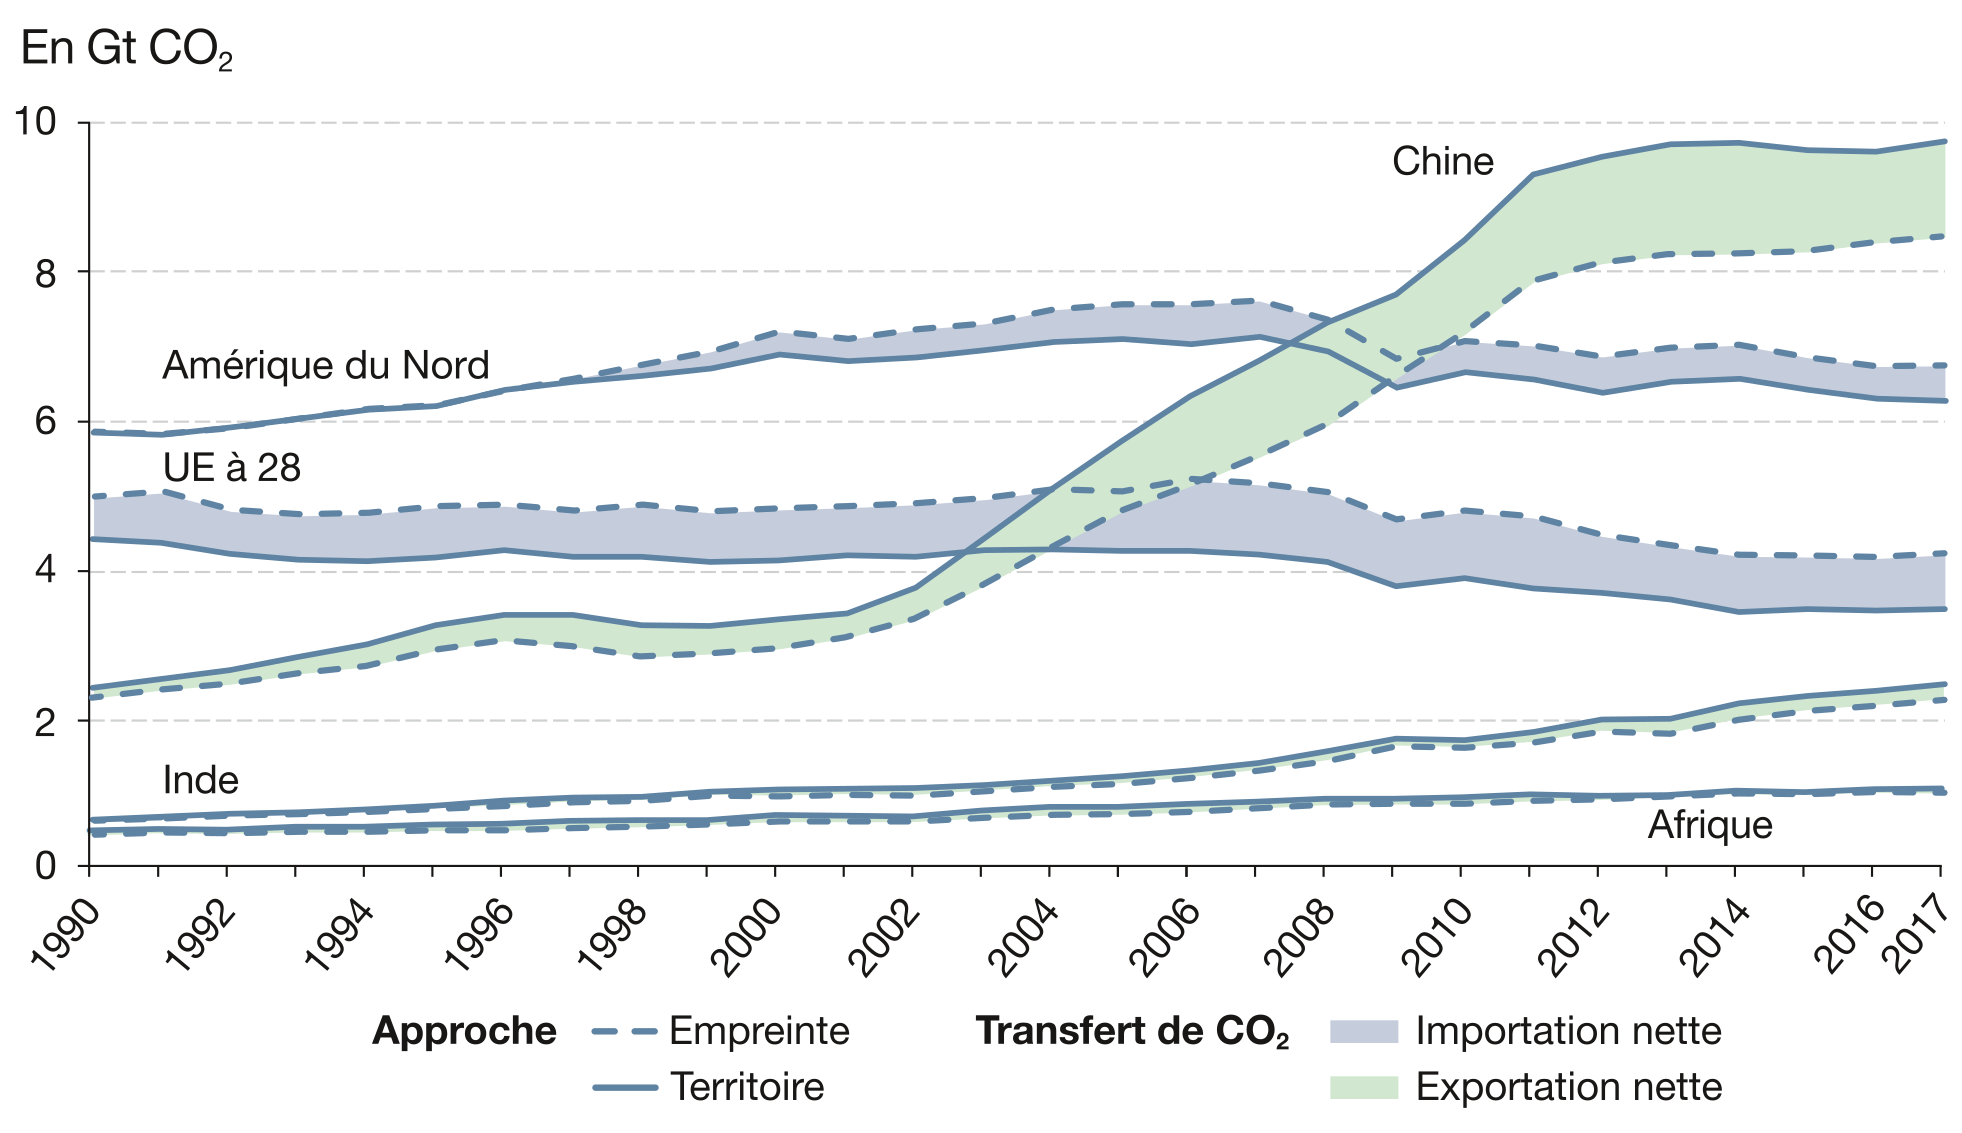
\includegraphics{img/comparaison-internationale-emissions-CO2-CGDD.png}

C'est une bonne nouvelle, mais en 2008 il se produit 2 événements :

\begin{enumerate}
\def\labelenumi{\arabic{enumi}.}
\tightlist
\item
  La crise des Subprimes entraînant un fort ralentissement des
  investissements.
\item
  Le passage symbolique des 100 dollar US avec un record de 147 le 11
  juillet 2008
  \emph{\href{https://prixdubaril.com/comprendre-petrole-cours-industrie/68508-grandes-hausses-baisses-prix-petrole-1990-2020.html\#:~:text=En\%20janvier\%202008\%2C\%20le\%20baril,2008\%2C\%20d\%C3\%A9passant\%20les\%20147\%20dollars.}{3}}
  sur le prix du baril conduit à une adaptation des comportements
  individuels et au début des politiques environnementales;
\item
  Le franchissement du pic d'extraction de pétrole conventionnel
  \emph{\href{https://www.lemonde.fr/blog/petrole/2019/02/04/pic-petrolier-probable-dici-a-2025-selon-lagence-internationale-de-lenergie/}{4}}
  selon l'IAE.
\end{enumerate}

On peut affirmer que depuis 2008, l'UE subit une décroissance de ses
émissions intérieures de CO2, sûrement due à la diminution des
extractions de pétrole conventionnel. Il faut aussi noter que, selon le
rapport de 2018 de l'IAE, le pic de production pétrolière global est
estimé à 2025
\emph{\href{https://www.lemonde.fr/blog/petrole/2019/02/04/pic-petrolier-probable-dici-a-2025-selon-lagence-internationale-de-lenergie/}{4}},
le consensus s'accorde sur une date comprise entre 2025 et 2030.

\begin{quote}
Note : Le pétrole dit conventionnel est le résultat de l'extraction
directe par forage dans un réservoir de pétrole. Le pétrole dit non
conventionnel couvre tous les autres types d'extraction (ex: pétrole de
schiste et schiste bitumineux.)
\end{quote}

Ainsi, que nous le décidions ou non, il faudra toujours faire avec moins
de pétrole. En effet, le pétrole non-conventionnel ne s'exporte que très
peu, tout comme le charbon.

En zoomant sur la France et en s'intéressant sur la répartition de nos
émissions de \(CO_2\) on remarque :\\
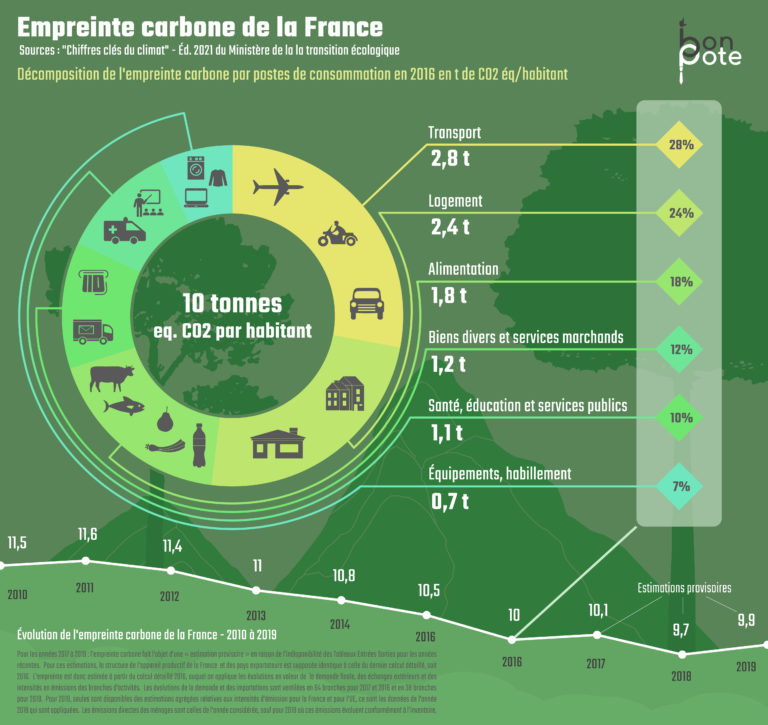
\includegraphics{img/1.Empreinte-carbone-1-768x725.jpg}

\begin{itemize}
\tightlist
\item
  10\% de nos émissions sont hors de notre champ d'action
  \emph{\href{https://bonpote.com/les-infographies-bon-pote/}{1}}
\item
  90\% restant se répartissent de la façon suivante
  \emph{\href{https://bonpote.com/les-infographies-bon-pote/}{1}} :

  \begin{enumerate}
  \def\labelenumi{\arabic{enumi}.}
  \tightlist
  \item
    Transport (31\%).
  \item
    Logement (27\%).
  \item
    Alimentation (20\%).
  \item
    Bien et service (14\%).
  \item
    Équipements et habillement (8\%).
  \end{enumerate}
\end{itemize}

Deuxième bonne nouvelle:

\begin{itemize}
\tightlist
\item
  nous pourrions agir directement sur 90\% de nos émissions de \(CO_2\),
  ce qui est de bonne augure pour descendre à \(2 tCO_{2eq}/hab\) comme
  la actée la COP de paris en 2015.
\end{itemize}

Cependant le cabinet de conseil Carbone 4 dans son rapport \emph{Faire
sa part ?} estime qu'un engagement dit `héroïque', avec des
investissements pour décarboner son mode vie, ne permet de diminuer que
de 45\% \href{https://www.carbone4.com/publication-faire-sa-part}{5}
l'empreinte carbone globale d'un français ou d'une française.

\hypertarget{chauffe-marcel}{%
\subsubsection{Chauffe Marcel}\label{chauffe-marcel}}

\begin{quote}
+5°C, la belle affaire ! On utilisera moins de pulls.
\end{quote}

Avec la COP 26, qui a eu lieu en 2021, les pays ont redit leur volonté
de limiter le réchauffement climatique à +2°C globaux pour 2100.
Cependant les COP ne sont que des accords de principe sans aucune
contrainte ou autorité de suivi.

Mais finalement que signifie 2, 3 ou 5°C de plus ?

Première mauvaise nouvelle :

\begin{itemize}
\tightlist
\item
  notre corps est un très mauvais thermomètre. Il est difficile pour lui
  de percevoir une variation de quelques degrés. De plus, on parle de
  température moyenne sur une échelle de temps de 3 siècles
  (\(XIX^{ème}\) - \(XXI^{ème}\)).
\end{itemize}

Une élévation moyenne de la température terrestre de 5°C s'est produite
entre -11 700 ans
\emph{\href{https://fr.wikipedia.org/wiki/Glaciation_de_W\%C3\%BCrm}{6}}
et le \(XIX^{ème}\) siecle. Au plus fort de la période glacière Würm, il
était possible de se rendre en Grande-Bretagne à pieds comme le montre
la carte ci-dessous :\\
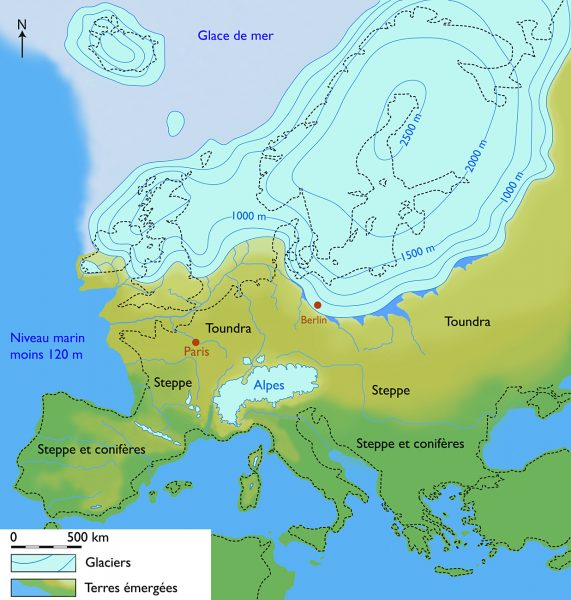
\includegraphics{img/10-Europe-au-LGM-571x600.jpg}

Cette évolution sur plus d'une dizaine de milliers d'années a permis une
augmentation du niveau de la mer de 120 m et le passage de paysages de
Toundra et de Steppes en France aux paysages que nous connaissons
actuellement.

Si on suit la trajectoire actuelle, la même élévation de température se
réalisera en l'espace de moins de 200 ans. Un tel réchauffement en un
laps de temps aussi court aurait des conséquences difficilement
imaginables. Si l'on regarde cette image, on voit que les conséquences
de la hausse de la température sur les changements environnementaux ne
sont pas proportionnelles. Ils sont exponentiels en fonction de la
température. Bien qu'une augmentation de 5°C ait de lourdes
conséquences, si l'on limite le réchauffement à 1,5 - 3°C, cela
suffirait pour diminuer l'impact de celui-ci sur la Terre.\\
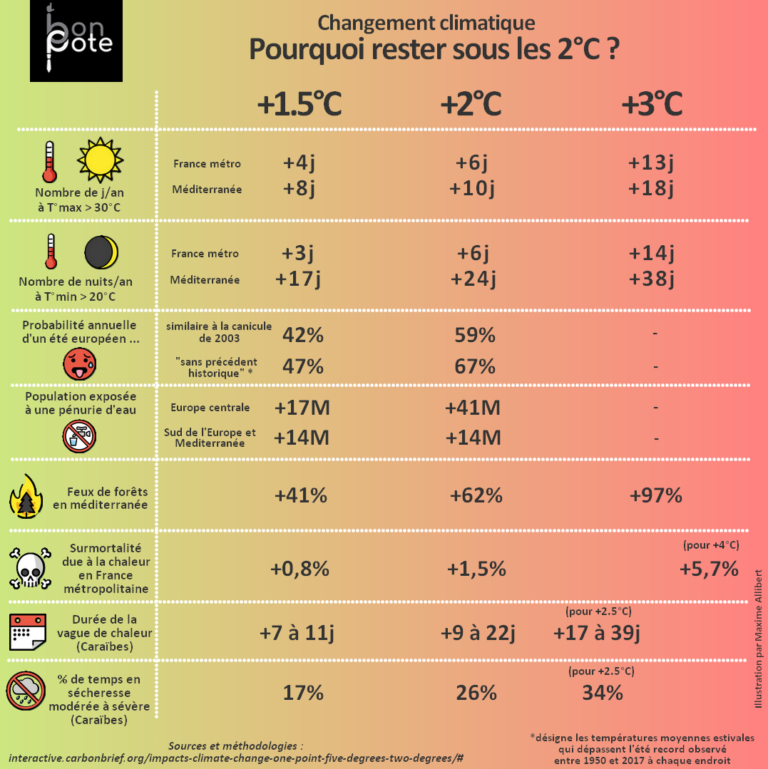
\includegraphics{img/Carbon_brief_test_15-768x769.png}

Dans cette illustration, en se focalisant uniquement sur la France et en
prenant une hausse de 1,5°C, nous avons :

\begin{itemize}
\tightlist
\item
  Presqu'une chance sur deux d'avoir une température moyenne estivale
  supérieure aux records enregistrés entre 1950 et 2017;
\item
  Plus de 2 semaines par an avec une température minimale la nuit
  supérieure à 20°C.
\end{itemize}

Tout degré de température supplémentaire implique un stockage de 20\% de
plus de vapeur d'eau dans l'atmosphère et celle-ci est le principal gaz
à effet de serre. C'est à cause d'elle que les changements globaux
augmentent de façon plus ou moins exponentielle avec la température.
Sans la vapeur d'eau on estime que la température de la terre serait de
-18°C
\emph{\href{https://www.futura-sciences.com/planete/questions-reponses/rechauffement-climatique-vapeur-eau-elle-gaz-effet-serre-912/}{8}}.
Heureusement le cycle de l'eau la fera retomber sur Terre, mais sous
forme de violentes pluies. De plus, le gradient de température entre le
sol (troposphère) et l'atmosphère (stratosphère), va s'accentuer, créant
ainsi des mouvements convectifs d'air, mouvements violents et plus
importants (cyclone, tornade, typhon\ldots).

Bonne nouvelle tout de même (enfin tout dépend où l'on se trouve),
l'Europe devrait mieux s'en sortir que les pays proches de l'équateur.
Là-bas, la température et le taux d'humidité extérieurs seront
suffisants pour que quiconque ne se trouvant pas dans un environnement
contrôlé, subisse la même mort que les personnes âgées lors de la
canicule de 2003
\emph{\href{https://www.lemonde.fr/climat/article/2017/06/19/mourir-de-chaud-un-risque-pour-30-de-la-population-mondiale_5147554_1652612.html}{7}}.\\
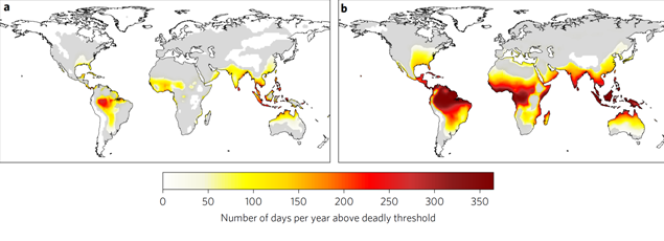
\includegraphics{img/ae0c102_12566-a1oldw.pq0pl7syvi.png}

La cartographie ci-dessus a été réalisée à partir des travaux du GIEC et
publiée dans une revue scientifique à comité de lecture \emph{Nature
Climate Change}. La cartographie \textbf{a} se base sur un scénario de
+1,5°C alors que l'autre sur un scénario de +5°C. Les morts surviendront
par défaut de régulation thermique, autrement dit l'être humain n'aura
plus la possibilité de réguler la température de son corps en en
évacuant la chaleur.

\hypertarget{section}{%
\subsubsection{2050}\label{section}}

Si on reprend le titre du livre de JM.Jancovici il faudrait plutôt dire
: \emph{Dormez tranquille jusque 2050}.

C'est la dernière bonne nouvelle, quel que soit le scénario que l'on
choisit. Réduire drastiquement les émissions ou continuer à vivre comme
aujourd'hui, le climat de 2050 est déjà écrit et connu.

\href{https://youtu.be/64xNugjI6jc}{Video quel climat en europe pour
2050 ?}

Pourquoi cette certitude ? Simplement parce que le système de régulation
climatique sur Terre possède une inertie. Si l'on veut bien comprendre
le phénomène, lorsque l'on arrête d'alimenter les fourneaux d'une usine,
ils continuent à chauffer jusqu'à ce que le liquide ou le gaz
refroidisse. Plus les usines sont grosses, plus il y a une grosse
quantité de liquide ou de gaz à faire refroidir, ce qui est plus long.
Imaginez le temps qu'il faut pour notre bonne vieille Terre, qui est
entourée de gaz ! De plus, quand on relâche une tonne de \(CO_2\) dans
l'atmosphère, 100 ans plus tard, il en reste encore au moins une
demi-tonne
\emph{\href{https://jancovici.com/changement-climatique/gaz-a-effet-de-serre-et-cycle-du-carbone/quels-sont-les-gaz-a-effet-de-serre-quels-sont-leurs-contribution-a-leffet-de-serre/}{9}}.

Vous ne verrez pas de votre vivant les effets de vos actions de
réduction de l'émission de CO2. Mais les générations futures les
verront. Il faut profiter de cette fenêtre de tir ou nous avons accès
`facilement' à l'énergie et vivons avec ``peu'' de contraintes
climatiques pour amorcer la transition.

\hypertarget{le-green-it-notre-sauveur}{%
\subsection{Le green IT notre sauveur}\label{le-green-it-notre-sauveur}}

\hypertarget{les-origines-10}{%
\subsubsection{\texorpdfstring{Les origines
\emph{\href{https://fr.wikipedia.org/wiki/Informatique_durable\#Historique}{10}}}{Les origines 10}}\label{les-origines-10}}

\begin{itemize}
\tightlist
\item
  1992 : Les Etats-Unis lancent le programme \emph{Energy star},
\item
  1998 : Tenue de la convention Aarthus qui définie le terme:
  information environnementale. Elle permet d'avoir accès a des données
  quantitatives et qualitatives sur l'environnement,
\item
  2003 : L'UE fixe les obligations des collectivités en matière de mise
  à disposition de l'information environnementale,
\item
  2004 : Fondation de la Fédération de la communauté francophone autour
  du GreenIT.fr,
\item
  2011 : Création de l'Alliance Green IT, association loi 1901 qui
  regroupe les acteurs français de l'informatique durable,
\item
  2012 : Publication de la première édition \emph{Ecoconception web :
  les 115 bonnes pratiques},
\item
  2015 : Appel à engagements pour la convergence entre les transitions
  écologique et numérique par le Conseil National du Numérique.
\end{itemize}

\hypertarget{en-pratique}{%
\subsubsection{En pratique}\label{en-pratique}}

Le green IT ne se focalise pas uniquement sur la tech ou le code. Toute
entreprise travaillant avec du matériel informatique peut appliquer des
mesures du green IT
\emph{\href{https://club.greenit.fr/doc/2017-12-ClubGreenIT-RefGIT-checklist.v2.pdf}{11}}.

Pour une ESN ou une société disposant d'un serveur, il est possible
d'estimer les émissions de \(CO_2\) qu'il produit : Sachant que les
serveurs actuels consomment une puissance moyenne de 170 W chacun
\emph{\href{https://normandie.ademe.fr/sites/default/files/chiffres-cles-consommation-energetique-equipements-informatiques.pdf}{12}}.
En prenant une hypothèse de fonctionnement d'un serveur sur toute
l'année, il consomme \(170 \cdot 365 \cdot 24 = 1 489 kWh/an\) . D'autre
part, 1 kWh d'électricité n'a pas la même empreinte carbone d'un pays à
l'autre. En effet, ceux-ci ne produisent pas l'électricité de la même
manière (pétrole, charbon, nucléaire, renouvelables\ldots{} avec des
parts différentes pour chaque moyen selon les pays).\\
En multipliant la production de \(CO_2\) (lors de la création
d'électricité) selon les pays par la consommation en kWh de d'un serveur
\emph{\href{https://www.bilans-ges.ademe.fr/documentation/UPLOAD_DOC_FR/index.htm?moyenne_par_pays.htm}{13}}
on obtient:

\begin{enumerate}
\def\labelenumi{\arabic{enumi}.}
\tightlist
\item
  Serveur français : \(89,34 kgCO_{2eq}\).
\item
  Serveur canadien : \(276,95 kgCO_{2eq}\).
\item
  Serveur chinois : \(610,49 kgCO_{2eq}\).
\item
  Serveur des Royaumes-Unis : \(680,47 kgCO_{2eq}\).
\item
  Serveur des Etats-Unis : \(777,26 kgCO_{2eq}\).
\end{enumerate}

Ainsi un serveur hébergé en France émettra presque 10 fois moins qu'un
même serveur hébergé aux Etats-Unis. Il est donc intéressant dans un
contexte de cloudification de choisir d'héberger ses applications sur
des serveurs dont le mix énergétique est faiblement émetteur de
\(CO_2\).

Quid alors de résilience en cas d'incendie ou de catastrophes. Quid
également du temps de latence.

\begin{enumerate}
\def\labelenumi{\arabic{enumi}.}
\tightlist
\item
  La résilience :

  \begin{enumerate}
  \def\labelenumii{\arabic{enumii}.}
  \tightlist
  \item
    choisir une architecture en micro-service et stocker les
    micro-services sur des partitions distinctes,
  \item
    sauvegarder les données dans une autre zone,
  \item
    provisionner des VM de secours.
  \end{enumerate}
\item
  La latence :

  \begin{enumerate}
  \def\labelenumii{\arabic{enumii}.}
  \tightlist
  \item
    concevoir des API qui envoient peu de données,
  \item
    respecter les bonnes pratiques de l'écoconception,
  \item
    proposer une expérience utilisateur qui permet d'attendre quelques
    secondes.
  \end{enumerate}
\end{enumerate}

En juin 2011, \emph{Le livre vert : Datacenters et Développement Durable
/ État de l'art et perspectives du Syntec numérique} indiquait :

\begin{quote}
L'optimisation au niveau serveur permet notamment un effet `cascade' ou
`boule de neige'.
\end{quote}

En réduisant les besoins de la couche logicielle, on réduit les besoins
en équipements informatiques et donc des systèmes d'alimentation et de
refroidissement. La consommation électrique du datacenter baisse alors
mécaniquement dans sa globalité. Cet effet cascade a un impact en phase
d'exploitation (sur la consommation électrique) mais également en phase
d'investissement. En effet, encore trop régulièrement, la construction
des salles serveurs est dimensionnée sur la base de puissance théorique
issue des fiches constructeurs
\emph{\href{https://www.ademe.fr/sites/default/files/assets/documents/guide-lecture-livre-blanc-consommation-energetique-2015.pdf}{14}}.\\
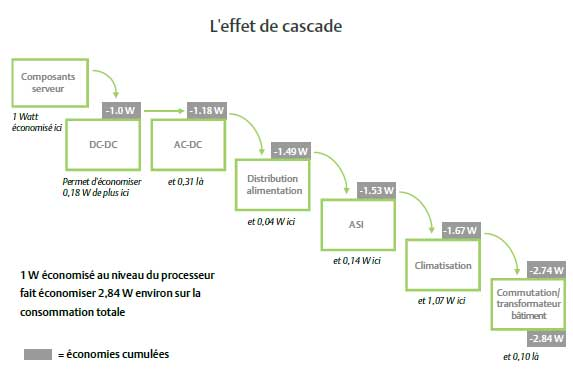
\includegraphics{img/effet-cascade.jpg}

\hypertarget{et-lhumain}{%
\subsubsection{Et l'humain}\label{et-lhumain}}

On a tendance à s'imaginer le sujet du Green-IT devant être traité par
les développeurs et les responsables infra. Or, le Green-IT c'est avant
tout des gestes que toute personne travaillant dans une société peut
faire. Ils sont nombreux mais on va s'attarder sur 2 gestes sur lesquels
seuls les collaborateurs ou collaboratrices peuvent agir directement :

\begin{itemize}
\tightlist
\item
  L'impression de documents :

  \begin{itemize}
  \tightlist
  \item
    une page imprimée (recto ou recto/verso) représente
    \(10,22 gCO_{2eq}\)
    \emph{\href{https://sites.google.com/site/pasdepapier/home/l-empreinte-carbone}{15}},
  \item
    l'utilisation d'une ramette de papier recyclé émet \(70 gCO_{2eq}\)
    de plus qu'une ramette issue d'arbre feuillus
    \emph{\href{https://www.bilans-ges.ademe.fr/documentation/UPLOAD_DOC_FR/index.htm?papier__carton_et_articles_en_.htm}{16}},
  \item
    n'imprimer que ce qui est nécessaire.
  \end{itemize}
\item
  Le mode de transport domicile-travail pour un trajet de 10km
  \emph{\href{https://monimpacttransport.fr/}{17}} :

  \begin{itemize}
  \tightlist
  \item
    un trajet seul en voiture émet \(198 gCO_{2eq}\),
  \item
    un trajet en métro émet \(25 gCO_{2eq}\),
  \item
    un trajet en vélo à assistance électrique \(20 gCO_{2eq}\) (si
    musculaire alors \(0 gCO_{2eq}\)).
  \end{itemize}
\end{itemize}

En prenant l'exemple d'une ESN qui travaille sur le développement d'une
application sur un sprint de 2 semaines et en prenant les hypothèses
suivante :

\begin{itemize}
\tightlist
\item
  une personne de l'administration est nécessaire pour 40 personnes,
\item
  l'équipe de développement se compose de 2 développeu·r·se·s,
\item
  une personne du management est nécessaire pour 6 développeu·r·se·s,
\item
  tout le monde vient en voiture.
\end{itemize}

En données d'entrée on prendra pour les véhicules :

\begin{longtable}[]{@{}
  >{\raggedright\arraybackslash}p{(\columnwidth - 8\tabcolsep) * \real{0.0935}}
  >{\centering\arraybackslash}p{(\columnwidth - 8\tabcolsep) * \real{0.2336}}
  >{\raggedright\arraybackslash}p{(\columnwidth - 8\tabcolsep) * \real{0.1028}}
  >{\centering\arraybackslash}p{(\columnwidth - 8\tabcolsep) * \real{0.2523}}
  >{\centering\arraybackslash}p{(\columnwidth - 8\tabcolsep) * \real{0.3178}}@{}}
\toprule
\begin{minipage}[b]{\linewidth}\raggedright
Modèle
\end{minipage} & \begin{minipage}[b]{\linewidth}\centering
Consommation \(l/100km\)
\end{minipage} & \begin{minipage}[b]{\linewidth}\raggedright
Carburant
\end{minipage} & \begin{minipage}[b]{\linewidth}\centering
Émission \(gCO_{2eq}/100km\)
\end{minipage} & \begin{minipage}[b]{\linewidth}\centering
Émission carburant \(gCO_{2eq}/l\)
\end{minipage} \\
\midrule
\endhead
fiesta & 7,3
\emph{\href{https://fr.mappy.com/itineraire\#/option_de_deplacement}{18}}
& essence & 99
\emph{\href{https://www.lacentrale.fr/fiche-technique-auto.php}{19}} &
507
\emph{\href{https://www.bilans-ges.ademe.fr/documentation/UPLOAD_DOC_FR/index.htm?new_liquides.htm}{20}} \\
308 & 5,6
\emph{\href{https://fr.mappy.com/itineraire\#/option_de_deplacement}{18}}
& diesel & 108
\emph{\href{https://www.lacentrale.fr/fiche-technique-auto.php}{19}} &
543
\emph{\href{https://www.bilans-ges.ademe.fr/documentation/UPLOAD_DOC_FR/index.htm?new_liquides.htm}{20}} \\
X3 & 9,4
\emph{\href{https://fr.mappy.com/itineraire\#/option_de_deplacement}{18}}
& essence & 239
\emph{\href{https://www.lacentrale.fr/fiche-technique-auto.php}{19}} &
507
\emph{\href{https://www.bilans-ges.ademe.fr/documentation/UPLOAD_DOC_FR/index.htm?new_liquides.htm}{20}} \\
\bottomrule
\end{longtable}

\begin{quote}
Note : Pour convertir des Giga Joules d'énergie en litre de carburant il
a été pris comme hypothèse de densité énergétique pour l'essence et le
diesel est de \(0,027 GJ/m^3\)
\emph{\href{https://www.convertir-unites.info/convertir+GJ+en+m3+Essence.php}{21}}.
\end{quote}

\begin{itemize}
\tightlist
\item
  \textbf{Impact Dominique (admin)} :

  \begin{itemize}
  \tightlist
  \item
    50 pages : \(\frac{50 \cdot 10,22}{1000} = 0,51 kgCO_{2eq}\)
  \item
    Trajet A-R 62km en peugeot 308 :
    \(62 \frac{5,6 \cdot (0,543 + 0,108)}{100} = 2,26 kgCO_{2eq}\)
  \item
    10 jours sur site : \(10 \cdot 2,26 = 22,60 kgCO_{2eq}\)
  \item
    Total : \(0,51 + 22,60 = 23,11 kgCO_{2eq}\)
  \end{itemize}
\item
  \textbf{Impact Raphaël (dev)} :

  \begin{itemize}
  \tightlist
  \item
    1 page : \(\frac{10,22}{1000} = 0,01 kgCO_{2eq}\)
  \item
    Trajet A-R 42km en ford fiesta :
    \(42 \frac{7,3 \cdot (0,507 + 0,099)}{100} = 1,86 kgCO_{2eq}\)
  \item
    8 jours sur site : \(8 \cdot 1,85 = 14,88 kgCO_{2eq}\)
  \item
    Total : \(0,01 + 14,88 = 14,89 kgCO_{2eq}\)
  \end{itemize}
\item
  \textbf{Impact Emmanuel (manager)} :

  \begin{itemize}
  \tightlist
  \item
    5 pages : \(\frac{5 \cdot 10,22}{1000} = 0,05 kgCO_{2eq}\)
  \item
    Trajet A-R 70km en BMW X3 :
    \(70 \frac{9,4 \cdot (0,507 + 0,239)}{100} = 4,91 kgCO_{2eq}\)
  \item
    8 jours sur site : \(8 \cdot 4,91 = 39,28 kgCO_{2eq}\)
  \item
    Total : \(0,05 + 39,28 = 39,33 kgCO_{2eq}\)
  \end{itemize}
\end{itemize}

À l'issue d'un sprint de 2 semaines cette équipe aura généré à elle
seule, en ne comptant que son transport et sa consommation de papier :
\(\frac{3}{40} \cdot 23,11 + 3 \cdot 14,89 + \frac{3}{6} \cdot 39,33 = 66,07 kgCO_{2eq}\)
soit presque 3/4 des émissions de CO2 d'un serveur hébergé en France
pendant 1 an.

\hypertarget{vous}{%
\subsection{Vous}\label{vous}}

\hypertarget{se-situer}{%
\subsubsection{Se situer}\label{se-situer}}

Sur internet, dans les médias ou autour de discussions, on peut trouver
de nombreux conseils et des idées pour réduire son empreinte carbone.
Mais bien souvent, il n'est pas évident de savoir l'impact réel de
chacun des petits gestes ou même d'en avoir un ordre de grandeur. Voici
donc une liste non exhaustive avec des exemples pour se situer :

\begin{itemize}
\tightlist
\item
  \textbf{La température de son logement}, les normes des performances
  énergétiques des bâtiments (RT2005, RT2012 et RE2020), imposent comme
  hypothèse de calcul, une température moyenne annuelle du logement à
  19°C
  \emph{\href{http://www.planbatimentdurable.fr/comprendre-la-rt-2012-r174.html}{22}}.
  Mais baisser son thermostat de 1°C représente une économie de 7\% de
  sa consommation d'énergie
  \emph{\href{https://librairie.ademe.fr/changement-climatique-et-energie/998-40-trucs-et-astuces-pour-economiser-l-eau-et-l-energie-9791029712784.html\#/44-type_de_produit-format_electronique}{23}}.
\item
  \textbf{La voiture}, les émissions varient beaucoup d'une énergie à
  une autre, d'une voiture à une autre, du pilote, etc. Mais on peut
  partir sur une moyenne de \(99 gCO_{2eq}\)
  \emph{\href{https://monimpacttransport.fr/}{17}} pour 5 km :

  \begin{itemize}
  \tightlist
  \item
    avoir un ou des passagers permet de répartir cette émission en parts
    égales,
  \item
    un trajet à vélo à 15 km/h prend 20 min
    (\(\frac{5}{15/60} = 20 min\)) en supprimant les émissions,
  \item
    un trajet à pied à 7 km/h prend 43 min (\(\frac{5}{7/60} = 43 min\))
    en supprimant les émissions.
  \end{itemize}
\item
  \textbf{L'avion}, il a révolutionné le transport entre les continents
  et permet de faire un Lille-Marseille en 1 h 35 min. Cela dit,
  l'émission par passager est de \(184,3 kgCO_{2eq}\)
  \emph{\href{https://monimpacttransport.fr/}{17}}

  \begin{itemize}
  \tightlist
  \item
    un trajet en TGV prendra approximativement 3 fois plus de temps (5 h
    08 min) en divisant d'un facteur 84 les émissions
    (\(2,20kgCO_{2eq}\)) selon la SNCF;
  \item
    un trajet en voiture avec un passager prendra 6,5 fois plus de temps
    (9 h 45 min) en divisant par moins de 2 les émissions par rapport à
    l'avion (\(96,60kgCO_{2eq}\))
    \emph{\href{https://monimpacttransport.fr/}{17}}
  \end{itemize}
\item
  \textbf{Les déchets}, ils génèrent également des gaz à effets de
  serres (GES) de par leurs transports. Pour les ordures ménagères il
  faut y ajouter le cycle de traitement (incinération ou enfouissement)
  soit \(707,67 kgCO_{2eq}\)
  \emph{\href{https://nosgestesclimat.fr/documentation}{24}} :

  \begin{itemize}
  \tightlist
  \item
    en achetant un maximum en vrac et en compostant des déchets
    organiques, on réduit de 2/3 nos émissions
    \emph{\href{https://nosgestesclimat.fr/documentation}{24}},
  \item
    en faisant ses produits ménagers et cosmétiques, en achetant des
    produits 100\% ou majoritairement réutilisables les émissions sont
    divisés par 3
    \emph{\href{https://nosgestesclimat.fr/documentation}{24}}.
  \end{itemize}
\item
  \textbf{L'électroménager et numérique}, les étiquettes énergétiques
  changent régulièrement. Depuis mars 2021, les notes vont à nouveau de
  A à F avec des seuils relevés. Ainsi un appareil A+++ vendu avant 2021
  peut être classé B ou C
  \emph{\href{https://fr.label2020.eu/la-nouvelle-etiquette-energie/caracteristiques-principales-des-nouvelles-etiquettes-energie/}{25}}.
  Puisque la production d'électricité est faiblement carbonée en France,
  les émissions de GES sont principalement dues à la production de ces
  appareils :

  \begin{itemize}
  \tightlist
  \item
    Pour un foyer de 3 personnes (2 adultes et un·e ado)
    l'électro-ménager, avant même d'avoir servi, a émis (en moyenne)
    \(1,79 tCO_(2eqs)\)
    \protect\hyperlink{Tableau-impact-fabriction}{cf}. Il est donc
    préférable qu'il soit amorti dans le temps. Pour cela, il faut
    garder et réparer ses appareils le plus longtemps possible (Le Black
    Friday n'est vraiment pas votre meilleur allié).
  \end{itemize}
\item
  \textbf{Le régime alimentaire}, sûrement le geste avec le rapport
  investissement/réduction le plus élevé. La production de viande de
  bœuf est la plus émettrice de GES (\(CH_{4}\) et \(CO_{2}\)). En
  effet, un bœuf demande beaucoup d'espace et de nourriture. Bien
  souvent, cette dernière est importée de très loin, faisant ainsi
  grimper l'empreinte carbone de la production de viande.

  \begin{itemize}
  \tightlist
  \item
    1kg de viande rouge produit en moyenne \(35,80 kgCO_{2eq}\),
  \item
    1kg de poisson blanc produit en moyenne \(9,59 kgCO_{2eq}\),
  \item
    1kg de volaille produit en moyenne \(5,16 kgCO_{2eq}\),\\
  \item
    1kg de poisson gras produit en moyenne \(4,03 kgCO_{2eq}\),
  \item
    1kg d'œuf produit en moyenne \(2,61 kgCO_{2eq}\),
  \item
    1kg de tofu produit en moyenne \(0,98 kgCO_{2eq}\).
  \end{itemize}
\end{itemize}

\begin{quote}
Note : Niveau nutritionnel, seul un régime 100\% végétalien (céréales,
légumineuses, fruits et légumes) comporte des risques de carence en
vitamine B12, zinc et fer. Pour les personnes anémiées en fer, il peut
être dangereux de se passer de viande rouge car cet aliment contient
beaucoup de fer facilement assimilable
\emph{\href{https://www.lemonde.fr/les-decodeurs/article/2021/02/27/non-il-n-est-pas-necessaire-de-manger-de-la-viande-pour-etre-en-bonne-sante_6071378_4355770.html}{26}}.
\end{quote}

\begin{figure}
\centering
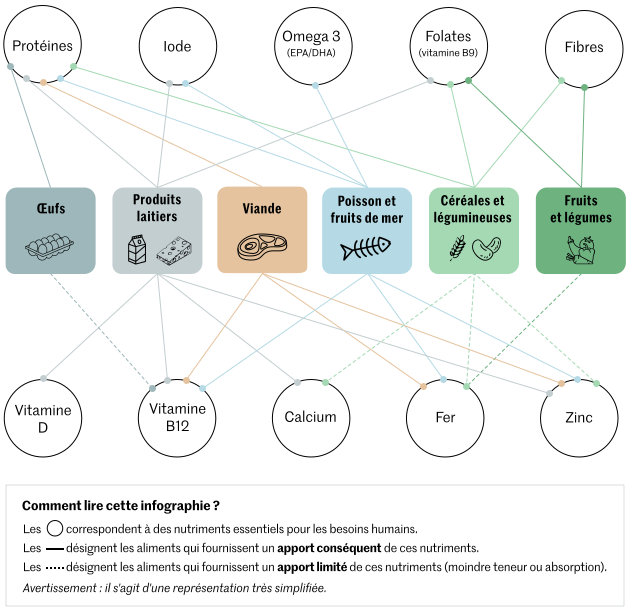
\includegraphics{img/infog2.png}
\caption{Apports nutritionnels des principaux aliments}
\end{figure}

\hypertarget{tableau-impact-fabriction}{%
\paragraph{Tableau impact fabriction}\label{tableau-impact-fabriction}}

\begin{longtable}[]{@{}lrc@{}}
\toprule
Appareil & Émission (\(kgCO_{2eq}\)) & Quantité \\
\midrule
\endhead
Réfrigérateur-congélateur & 25,70 & 1 \\
Lave-linge & 34,20 & 1 \\
Sèche-linge & 26,60 & 1 \\
Lave-vaisselle & 27,10 & 1 \\
Four & 18,08 & 1 \\
Micro-onde & 8,20 & 1 \\
Plaques & 6,53 & 1 \\
Bouilloire & 1,65 & 1 \\
Cafetière & 5,32 & 1 \\
Aspirateur & 6,55 & 1 \\
Robot cuisine & 41,30 & 1 \\
Appareil photo & 30,00 & 1 \\
Ordinateur portable & 156,00 & 2 \\
Tour ordinateur & 296,00 & 1 \\
Écran ordinateur & 248,00 & 1 \\
Home cinéma & 133,00 & 1 \\
Nokia 3310 & 16,50 & 0 \\
Smartphone & 39,10 & 2 \\
Iphone XI & 57,00 & 3 \\
Tablette & 63,00 & 1 \\
TV & 371,00 & 1 \\
Vidéo Projecteur & 94,00 & 0 \\
\bottomrule
\end{longtable}

\hypertarget{des-bonnes-intentions-mais}{%
\subsubsection{Des bonnes intentions
mais}\label{des-bonnes-intentions-mais}}

Toute action permettant de réduire nos émissions est bonne à prendre.
Seulement face au défis du réchauffement il faut avoir le sens des
priorités. Voici une liste de gestes dont on entend parler mais qui
n'ont qu'un impact minim sur nos émissions:

\begin{itemize}
\tightlist
\item
  \textbf{Faire confiance aux labels `verts'} requiert des connaissances
  précises sur les critères utilisés et sur le degré de contraintes
  imposées par l'autorité qui délivre ce label. Un label n'est jamais
  obligatoire, il est souvent utilisé dans un but commercial. Prenons
  l'exemple du label AB: Pour un produit alimentaire, il garantit qu'au
  moins 95\% des ingrédients sont d'origine agricole biologique
  \emph{\href{https://www.agencebio.org/wp-content/uploads/2018/10/regles_usage_marque_AB.pdf}{27}}
  et sont produits dans l'UE. Ainsi une tomate génétiquement
  sélectionnée pour sa résistance et poussant dans une serre chauffée au
  gaz en hiver en Espagne pourra apposer le label AB. Il peut être plus
  intéressant de réduire la chaîne d'approvisionnement en achetant au
  plus proche du producteur (en circuit court).\\
\item
  \textbf{Domotiser son logement} semble être une bonne solution pour
  faire des économies d'énergie. Cependant, comme l'électricité en
  France est bas carbone, cette action a des conséquences très faibles
  sur l'émission des GES. Cette solution est même assez dommageable en
  certains points puisqu'il faut acheter un boîtier propriétaire afin
  d'utiliser les solutions constructeurs. Celui-ci doit rester en
  fonctionnement en permanence. Il faut ajouter à cela, l'achat de
  nouvelles ampoules ou autres appareils électroniques compatibles. La
  domotique est néanmoins intéressante pour piloter son chauffage à
  distance par exemple. Grâce à elle, il est aussi plus simple
  d'utiliser ses appareils lorsque les éventuels pics de consommation
  d'énergie sont passés.\\
\item
  \textbf{Remplacer sa voiture} par une hybride rechargeable ou un
  SUV/Cross-over ayant une étiquette supérieure ou égal à B est
  intéressant uniquement si l'ancien véhicule a plus de 10 ans, ou plus
  de 210 000 km ou si son gabarit est supérieur ou égal à la nouvelle.
  En effet, les batteries ajoutent du poids au véhicule. Se déplacer
  demande alors plus d'énergie (\(E_{c}=\frac{m \cdot v^2}{2}\)). Enfin,
  le coefficient de pénétration dans l'air d'un SUV/Cross Over est bien
  plus élevé qu'un break par exemple.\\
\item
  \textbf{Passer du fioul au gaz pour le chauffage} apporte certes une
  réduction des GES, mais on remplace une énergie fossile par une autre
  qui n'est pas infinie. En fonction du budget et du type d'habitation,
  une chaudière à granulés, un poêle à bois, une pompe à chaleur ou des
  convecteurs électriques seront plus efficaces pour réduire les
  émissions de GES.\\
\item
  \textbf{Changer toutes ses ampoules fluo-compactes par des LED} ne
  permet qu'une faible économie de consommation (1\%)
  \emph{\href{https://www.carbone4.com/publication-faire-sa-part}{5}}.
  Il est préférable de remplacer les ampoules cassées ou les ampoules à
  filament ou encore les néons.
\end{itemize}

\begin{quote}
Note : En France il y a de nombreux organismes qui s'occupent de la
collecte et du recyclage de vos ampoules ou néons usagés.
\end{quote}

\begin{itemize}
\tightlist
\item
  \textbf{Choisir un fournisseur d'électricité verte} ne garantit en
  aucun cas que l'électricité arrivant dans le logement n'a pas émis de
  carbone. En effet, l'électricité courante dans le réseau n'appartient
  encore à aucun fournisseur. Rien ne prouve que celle que j'utilise est
  celle que mon fournisseur paiera.
\end{itemize}

\hypertarget{comment-ruxe9duire-son-empreinte-individuelle}{%
\subsection{Comment réduire son empreinte individuelle
?}\label{comment-ruxe9duire-son-empreinte-individuelle}}

Malheureusement, penser que réduire son impact sera facile, demandera ni
sacrifice ni investissement, est un leurre. La publication \emph{Faire
sa part} de carbone 4
\emph{\href{https://www.carbone4.com/publication-faire-sa-part}{5}} est
catégorique. Sans investissements financiers mais en réalisant des
changements radicaux de notre mode vie, on ne peut réduire que de 25\%
les émissions de GES. Ce taux descend à 10\% pour des changements dits
``réalistes''. Dans cette même publication, on peut constater que les
actions maximales activables par les ménages sans investissements sont
de :

\begin{itemize}
\tightlist
\item
  \(1,3 tCO_{2eq}\) pour l'alimentation (régime végétarien, achat local,
  zéro déchet et gourde),
\item
  \(0,9 tCO_{2eq}\) pour la mobilité (vélo pour trajet de moins 10km,
  100\% covoiturage, ne plus prendre l'avion),
\item
  \(0,5 tCO_{2eq}\) pour les biens et services (trois fois moins de
  vêtements neufs, électronique et hi-tech d'occasion),
\item
  \(0,2 tCO_{2eq}\) pour le logement (baisser la température de consigne
  et équiper son logement d'éclairage LED).
\end{itemize}

Par rapport aux \(10,8 tCO_{2eq}\) d'émission cela ne représente qu'une
baisse de 27\% en changeant considérablement son mode de vie.

En prenant ces propositions, ainsi que celle de l'ADEME et de
l'association négaWatt
\emph{\href{https://negawatt.org/IMG/pdf/synthese-scenario-negawatt-2022.pdf}{29}},
on peut arriver à répertorier les vrais gestes, actions et
investissements à réaliser pour faire diminuer les émissions de GES.

\begin{quote}
Note : le scénario négaWatt de 2022 suppose une sobriété accrue des
ménages et des industries (diminution de notre consommation de pétrole
dans notre quotidien qui est difficilement acceptable par la société).
En outre, il pose des hypothèses sur les technologies récentes mais
n'ayant pas été développé à l'échelle industrielle. Elle omet aussi le
problème de concurrence d'utilisation des sols.
\end{quote}

\hypertarget{les-premiers-gestes}{%
\subsection{Les premiers gestes}\label{les-premiers-gestes}}

\begin{itemize}
\tightlist
\item
  Connaître son empreinte carbone actuelle sur
  \href{https://nosgestesclimat.fr/}{NosGestesClimat} permet de faire un
  état de lieu de sa situation personnelle. Le site propose des actions
  et des défis à réaliser pour réduire son empreinte. Il est même
  possible d'apporter des améliorations avec un langage de programmation
  accessible.\\
\item
  Installer des thermostats programmables par zone d'occupation permet
  un pilotage au plus proche des besoins d'un foyer. En effet
  l'occupation d'un bureau ou de chambres n'est pas la même que celle
  d'une cuisine, d'un salon ou d'une salle de bain.\\
\item
  Covoiturer pour son trajet domicile-travail répartit entre les
  occupants le coût et les émissions engendrées par ce trajet. Ceci peut
  se cumuler également avec l'utilisation d'un vélo ou d'une trottinette
  électrique pour des trajets de moins de 5 km.\\
\item
  Prendre une carte de réduction à la SNCF peut paraître anecdotique
  mais cela nous incite à envisager le train à la place de la voiture ou
  de l'avion.\\
\item
  Éteindre ses appareils et ne pas laisser son ordinateur portable ou
  son smartphone sur le secteur permet d'éviter de gâcher de l'énergie.
  En l'absence de chargeurs dit ``intelligents'' capables de se couper
  automatiquement, l'utilisation de prises programmables est une
  solution pertinente.\\
\item
  Les labels étant nombreux et non obligatoires, seule l'origine des
  produits peut devenir un critère objectif d'émission de GES. Choisir
  son produit en fonction de la proximité de son origine et non selon le
  prix, permet d'affirmer que nous sommes sur la bonne voie.\\
\item
  \emph{Les antibiotiques, c'est pas automatique !} On peut paraphraser
  ce slogan \emph{Les viandes durant les repas, c'est pas systématique
  !}. La grande distribution a permis à une large majorité de français
  de manger de la viande au moins une fois par jour. Pourtant les
  éleveurs français ont subi une crise sans précédent. En allant vers
  des circuits courts on peut manger de la viande de meilleure qualité,
  peut-être moins souvent, mais cela vaut le coup si c'est pour redonner
  confiance à nos éleveurs.
\end{itemize}

\hypertarget{les-gestes-demandant-un-changement-de-mentalituxe9}{%
\subsection{Les gestes demandant un changement de
mentalité}\label{les-gestes-demandant-un-changement-de-mentalituxe9}}

\begin{itemize}
\tightlist
\item
  S'il est difficile, voire impossible, d'acheter de la viande en
  circuit court et s'il n'y a pas de contre indications médicales, il
  est envisageable de réserver la viande uniquement aux restaurant ou
  chez des amis. Évidemment on peut choisir cette option directement par
  conviction.\\
\item
  Se fixer un objectif d'émissions de CO2 annuel est un bon moyen pour
  gérer sa mobilité. Cet objectif doit être atteignable et dépend de
  votre localisation.
  \href{https://monimpacttransport.fr/}{MonImpactTransport} et/ou des
  calculs au réel en utilisant le \protect\hyperlink{et-lhumain}{tableau
  données d'entrées des véhicule} ainsi que les émissions du véhicule
  (V.7 sur la carte grise), permettent de suivre vos émissions tout au
  long de l'année.\\
\item
  Se passer des grandes surfaces serait l'idéal mais se limiter
  uniquement aux produits non alimentaires est déjà un grand pas.
  Attention toutefois aux achats en ligne et aux grossistes qui vendent
  des produits qui ne sont pas de saisons.\\
\item
  Une bonne tartiflette c'est bon et c'est encore meilleur lorsqu'on l'a
  faite soi-même. Ce peut-être le cas aussi pour le pain, mais
  attention, il ne faut pas tomber dans l'écueil du 100\% home made et
  acheter du matériel faisant grimper l'empreinte de l'équipement
  électro-ménager.\\
\item
  La réutilisation est très bien pour diminuer l'empreinte carbone des
  biens et des services. Cependant certains objets du quotidien vont se
  heurter à notre acceptabilité. Si les couches, serviettes hygiéniques
  et culottes menstruelles lavables font leur chemin, sommes nous tous
  prêts à les utiliser. Pour certains, il y a u bloquage psychologique à
  ne pas négliger. De plus, certaines choses sont difficilement
  remplçables par du durable. En effet, pourrons-nous nous passer de
  papiers-toilettes, sommes nous prêt à nous essuyer les fesses avec du
  tissu et à passer notre temps à le laver ?\\
\item
  Le sèche linge rend beaucoup de services, mais n'est pas nécessaire si
  un logement disposant d'un espace extérieur et intérieur pour faire
  sécher le linge existe, même si, parfois, les pulls mettent plusieurs
  jours à sécher. La même question peut se poser sur la télévision, à
  l'heure des portails de VOD, YouTube, Twitch, etc\ldots{} Revendre sa
  télévision et acheter un projecteur émettant 4 fois moins de CO2 peut
  s'avérer être une bonne idée.\\
\item
  En parler avec ses proches pour les sensibiliser est peut-être la
  chose la plus difficile car on se heurte à l'acceptabilité et aux
  certitudes des autres. Cela demande de la pédagogie et de l'empathie.
\end{itemize}

\hypertarget{investir-pour-duxe9carboner}{%
\subsection{Investir pour
décarboner}\label{investir-pour-duxe9carboner}}

\hypertarget{le-logement}{%
\subsubsection{Le logement}\label{le-logement}}

Dès 2023 les logements de classe G ne pourront plus être loués. Même
pour un logement classé D ou E, il est pertinent d'investir dans une
rénovation thermique globale. Il y a cependant un ordre à respecter :

\begin{enumerate}
\def\labelenumi{\arabic{enumi}.}
\tightlist
\item
  Isolation avec des matériaux biosourcés (Tout sauf laine de verre,
  laine de roche et polystyrènes) :

  \begin{enumerate}
  \def\labelenumii{\arabic{enumii}.}
  \tightlist
  \item
    Toiture,
  \item
    Murs donnant sur l'extérieur,
  \item
    Plancher bas,
  \item
    Huisserie.\\
  \end{enumerate}
\item
  Production de chaleur :

  \begin{enumerate}
  \def\labelenumii{\arabic{enumii}.}
  \tightlist
  \item
    Remplacer la chaudière gaz/fioul par une pompe à chaleur, un
    radiateur à inertie sèche ou une chaudière à bois,
  \item
    Remplacer le ballon d'eau chaude par un chauffe-eau solaire et
    électrique.\\
  \end{enumerate}
\item
  Autres logements :

  \begin{enumerate}
  \def\labelenumii{\arabic{enumii}.}
  \tightlist
  \item
    Faire comme la résidence principale,
  \item
    Éviter que le logement ne reste vacant pour rentabiliser
    l'investissement.
  \end{enumerate}
\end{enumerate}

\begin{quote}
Note : Le mix énergétique d'électricité étant bas carbone,
l'installation de mini-centrales électriques ENR n'est, dans la plus
part des cas, pas pertinente en France. Elle peut le devenir si
l'électricité produite sert à recharger les batteries d'une voiture,
d'un vélo, d'une trottinette électrique ou encore a alimenter en
électricité un chauffe-eau.
\end{quote}

\hypertarget{les-vuxe9hicules}{%
\subsubsection{Les véhicules}\label{les-vuxe9hicules}}

Il convient de se poser la question de la réelle utilité d'une seconde
voiture. Des solutions plus économiques existent : les vélos cargos à
assistance électrique,les mini voitures comme la TWIZY ou l'Ami. La
voiture principale doit être envisagée comme dernière solution pour un
déplacement. Évidemment dans certains cas la seconde voiture est
essentielle et aucune autre solution n'est envisageable.

Concernant le véhicule principal, il faut éviter les formules location
longue durée et voire la location avec option d'achat comme une
obligation d'achat, pour ne pas changer toujours de voitures et éviter
d'inciter à la production de nouvelles voitures. Tout comme les
appareils électroniques une voiture à une empreinte non négligeable à la
fabrication qu'il faut amortir. Les constructeurs dimensionnent leur
véhicule pour 20 ans ou 250 000km. Si le véhicule à moins de 10 ans, il
est urgent d'attendre avant de le changer, sauf si la famille s'agrandit
et que le véhicule ne répond pas au besoin de mobilité.

Lors du changement de véhicule, il faut privilégier une motorisation
100\% électrique, mais il faut aussi choisir un modèle léger dont la
pénétration dans l'air est optimisée. Dans le cas d'une motorisation
partiellement ou entièrement thermique, il faut chercher à diminuer le
poids et à augmenter l'aérodynamisme du véhicule. Le dernier point à
prendre en compte sont les options qui doivent répondre à un critère
d'utilité et de la configuration du véhicule.

En résumé, il faut déconstruire l'image que l'on se fait de la voiture
comme un marqueur social. Une voiture doit rester un mode de locomotion
permettant de parcourir une longue distance infaisable à pied ou à vélo
et dont les solutions de mobilité partagées (bus, métro, ter, rer, tgv,
avion\ldots) ne peuvent répondre aux besoins.

\hypertarget{la-biodiversituxe9}{%
\subsection{La biodiversité}\label{la-biodiversituxe9}}

Si le réchauffement climatique est, à présent, relayé dans les médias et
la presse, la perte de la biodiversité est rarement considérée comme un
problème équivalent à celui des émissions de GES. Mais si l'on réduit
effectivement les émissions de GES pour suivre les recommandations du
GIEC, il reste encore le problème de la diminution de l'Indice de
Planète Vivante (IPV) dont seules quelques personnes ont entendu parler.
Pour bien se rendre compte des conséquences de la perte du vivant sur
notre planète, il y a l'excellent atelier: la fresque de la biodiversité
\emph{\href{https://www.fresquedelabiodiversite.org/}{30}} dont il est
recommandé d'y participer.

\hypertarget{quelques-chiffres}{%
\subsubsection{Quelques chiffres}\label{quelques-chiffres}}

L'IPV est utilisé par de nombreux organismes gouvernementaux et
inter-gouvernementaux. Il permet de suivre l'évolution du vivant sur
Terre. Cependant, il se base majoritairement sur les vertébrés sur
Terre, qui est le groupe le plus connu. Il calcule le taux de
décroissance (ou croissance) des populations de toutes les espèces
connues et en fait la moyenne. Depuis 1970, il a diminué de 68\% au
niveau mondial
\emph{\href{https://www.wwf.fr/rapport-planete-vivante}{31}}.

La France a une réelle responsabilité vis-à-vis de la préservation de la
biodiversité. En effet, 10\% des espèces connues dans le monde, vivent,
entre autres, en France (DROM-COM compris). On estime que 80\% de la
biodiversité vit en outre-mer. Mais pour l'instant, seules 85 238
espèces y sont connues contre 95 582 en métropole
\emph{\href{https://inpn.mnhn.fr/docs/communication/livretInpn/LIVRET_INPN_2019.pdf}{32}}.\\
Une particularité de la richesse en espèce d'une région, c'est qu'elle
est d'autant plus forte qu'elle est proche des tropiques. A ce titre,
58\% des espèces métropolitaines françaises sont présentes dans les
Alpes-Maritimes
\emph{\href{https://inpn.mnhn.fr/docs/communication/livretInpn/LIVRET_INPN_2019.pdf}{32}}.
Dans les Hauts-de-France, nous avons peu de diversité, il est d'autant
plus important de la préserver.

Des chiffres en vrac
\emph{\href{https://inpn.mnhn.fr/docs/communication/livretInpn/LIVRET_INPN_2019.pdf}{32}}
:

\begin{itemize}
\tightlist
\item
  53 \% des plantes liées aux insectes déclinent,
\item
  22 \% de déclin moyen des 10 oiseaux granivores les plus communs,
\item
  9500 espèces et sous-espèces protégées sur le territoire Français
  selon l'INPN,
\item
  50\% de la surface des zones humides en France a disparu entre 1960 et
  1990 selon l'état des lieux des Zones Humides.
\end{itemize}

Les causes menaçant les espèces sont diverses et variées. Les plus
importantes sont la destruction des habitats (notamment par
l'urbanisation), la chasse (que ce soit par les chats ou par les
humains), la pollution des eaux, l'arrivée d'espèces invasives, la
présence de nombreux perturbateurs pour les espèces. Un bon exemple est
l'éclairage urbain. La nuit, les espèces y sont exposées et cela
perturbe leur cycle ou leurs repères en les assimilant à la lune. En
effet, 85\% du territoire est exposé à un niveau élevé de nuisance
lumineuse
\emph{\href{https://ofb.gouv.fr/actualites/un-nouvel-indicateur-pour-mesurer-la-pollution-lumineuse\#:~:text=Le\%20nouvel\%20indicateur\%20de\%20l,niveau\%20\%C3\%A9lev\%C3\%A9\%20de\%20pollution\%20lumineuse.}{33}}).

\hypertarget{dans-mon-jardin}{%
\subsubsection{Dans mon jardin}\label{dans-mon-jardin}}

\begin{itemize}
\tightlist
\item
  Les plantes ornementales sont très prisées dans les jardins mais elles
  sont souvent exotiques. Elles ne comptent donc pas dans la
  biodiversité locale. De plus, elles peuvent parfois être
  envahissantes. Il existe de nombreuses espèces locales esthétiques
  dont l'entretien dans un jardin sera des plus facile. Le site du
  Conservatoire Botanique National de Bailleul
  \emph{\href{https://www.cbnbl.org/grainotheque}{34}} (CBNBL) pour les
  Hauts-de-France propose une grainothèque permettant de planter des
  espèces d'intérêt écologique et patrimonial.\\
\item
  Les Espèces Exotiques Envahissantes (EEE) sont des espèces exotiques
  dont l'introduction par l'homme, volontaire ou fortuite, sur un
  territoire, menace les écosystèmes, les habitats naturels ou les
  espèces indigènes avec des conséquences écologiques, économiques et
  sanitaires négatives. Le danger de ces espèces est qu'elles accaparent
  une part trop importante des ressources dont les espèces indigènes ont
  besoin pour survivre, ou qu'elles se nourrissent directement des
  espèces indigènes
  \emph{\href{https://www.ecologie.gouv.fr/especes-exotiques-envahissantes}{35}}.
  Ces espèces doivent être éliminées entièrement car un simple rhizome
  restant peut leur permettre de repartir. Seules certaines décharges
  vertes sont habilitées à les détruire.\\
\item
  Il est inutile de tondre toutes les deux semaines. Même si on trouve
  ça ``moche'', ceci découle de l'habitude de voir des pelouses tondues
  ras. Ne pas tondre trop souvent a pour avantage de laisser certaines
  plantes à cycle rapide faire des graines et des fleurs qui enrichiront
  le jardin. De plus, cela évitera aux autres espèces d'épuiser leurs
  ressources pour construire sans cesse de nouvelles feuilles.\\
\item
  Les plantes n'ont pas besoin d'eau potable et cette eau est rare.
  L'eau de pluie ne coûte rien et les plantes ne verront pas la
  différence.\\
\item
  La France est l'un des plus gros consommateurs d'engrais chimique en
  Europe. Par exemple, en 2018, 18 millions de tonnes de fertilisants
  minéraux et organiques ont été commercialisés en France métropolitaine
  dont 11,5 millions de tonnes d'origine minérale, selon l'Observatoire
  pour la fertilisation minérale et organique. Les engrais minéraux
  (chimiques) qui se déversent ensuite dans les cours d'eau, lors du
  ruissellement des pluies, perturbent la biodiversité ripicole.\\
\item
  Le compost est un fertilisant naturel. Pourquoi acheter des intrants
  chimiques et jeter les feuilles qui sont un intrant naturel
  lorsqu'elles se décomposent? De plus, elles amèneront une faune du sol
  variée et nombreuse, travaillant à leur transformation en humus.\\
\item
  Les insectes sont nécessaires à la pollinisation mais ils sont aussi à
  la base de nombreuses chaînes alimentaires. Ils ne se réduisent pas
  uniquement aux abeilles domestiques. Il est possible d'en favoriser de
  nombreux autres. Construire un hôtel à insectes est une activité
  ludique pour les enfants et elle les sensibilise à la protection de la
  nature.\\
\item
  L'hiver, de nombreux oiseaux ne migrent pas. Auparavant, ils pouvaient
  trouver assez facilement de la nourriture mais aujourd'hui, les
  espaces non construits se font rares et les populations d'espèces
  compétitives comme le pigeon, grandissent. Faire de petits nichoirs
  permet de favoriser les Mésanges, les Gros-bec, les Moineaux et
  d'autres passereaux.\\
\item
  Lorsque l'on cultive toujours au même endroit, le sol s'appauvrit au
  fur et à mesure. Bouger la serre permet de limiter l'utilisation
  d'intrants et de laisser le temps au sol de se recharger en matière
  organique se décomposant pour recréer de l'humus. Cet humus contient
  de la nourriture pour les plantes. Cela implique de ne pas laisser le
  sol sans végétation (les mauvaises herbes feront très bien
  l'affaire\ldots)
\end{itemize}

\hypertarget{dans-ma-maison-et-en-vacances}{%
\subsubsection{Dans ma maison et en
vacances}\label{dans-ma-maison-et-en-vacances}}

\begin{itemize}
\tightlist
\item
  Lorsque l'on construit une nouvelle maison passive, on agit pour la
  diminution des émissions de GES. Mais qu'en est-il des habitats
  naturels dont la surface diminue de plus en plus à cause de
  l'urbanisation? Cela entraîne immanquablement la diminution des
  populations d'espèces vivant dans ces habitats.\\
\item
  Apprendre à connaître la faune et la flore permet d'apprendre à
  prendre soin d'elle. Les scientifiques ont toujours besoin de données
  actualisées pour suivre l'évolution de la biodiversité. Ce peut être
  signaler la présence de hérissons, chauves-souris, écureuils dans son
  jardin auprès d'associations locales par exemple.\\
\item
  Les chauves-souris en France sont en déclin. Elles subissent l'assaut
  des lumières persistantes pendant la nuit. Elles peuvent parfois
  s'épuiser de nombreuses heures autour d'un lampadaire, cela menant à
  leur mort. En outre, elles sont méconnues et mal-aimées car des
  légendes les présentaient autrefois comme des créatures de l'ombre.
  Laisser les combles accessibles aux chauves-souris participe à leur
  sauvegarde. Elles pourront venir y hiverner. Dans tous les cas, tuer
  une de ces petites bêtes est interdit et répréhensible car elles sont
  protégées.\\
\item
  Les plantes et animaux exotiques peuvent devenir exotiques
  envahissants si les conditions climatiques leurs sont favorables. Par
  ailleurs, certaines peuvent aussi représenter un risque pour la santé
  publique.\\
\item
  La Terre n'est pas une poubelle. Les déchets sont très nombreux
  partout. Ils ont de nombreuses incidences sur la vie des espèces. On
  connaît très bien, notamment par les médias, les problèmes que
  subissent les poissons avec les plastiques dans les océans. C'est
  aussi le cas dans les rivières, ou pour les oiseaux. Ajoutons à cela
  que les papiers contiennent parfois des encres qui peuvent être des
  produits toxiques pour les espèces. Les produits dans les mégots de
  cigarette sont toujours toxiques quant-à-eux\ldots{} Les bouteilles
  sont des pièges pour de nombreux gastéropodes et pour la faune du sol.
  Chaque déchet jeté peut tuer plusieurs dizaines d'êtres vivants.
  Malheureusement, il y en a tellement que tous les ramasser semble une
  épreuve sans fin.\\
\item
  Le piétinement est une source de stress pour les plantes. Plus un
  espace est piétiné, moins il sera riche en espèces car il ne restera
  que les plus résistantes. Les animaux qui ont besoin de diversité sont
  liés aux habitats non piétinés. Pour éviter de trop impacter le
  vivant, autant limiter ce phénomène en se contentant de suivre le
  chemin.\\
\item
  Parfois une fleur peut être très belle, tellement que l'on voudrait la
  cueillir et la ramener chez soi. Pas de chance c'est une plante
  protégée! Leur destruction (et donc leur cueillette) est interdite et
  donc répréhensible. Pour permettre à ces espèces de se reproduire
  (pour ne pas disparaître), il faut les laisser accomplir leur cycle de
  reproduction complet (feuilles-fleurs-fruits-graines).\\
\item
  Certains médicaments contiennent des régulateurs hormonaux ou des
  substances toxiques pour les poissons. Après s'être retrouvées dans
  vos toilettes, ces substances sont emmenées dans les stations
  d'épuration. Mais, pour la plupart, les traitements qu'elles subissent
  ne les empêchent pas de se retrouver dans les rivières.\\
\item
  Privilégier la pêche durable est un moyen de garantir la reproduction
  suffisante des poissons en incitant les pêcheurs à respecter des taux
  de pêches plus faibles. Si une espèce se reproduit moins vite qu'elle
  n'est prédatée, elle disparaît.
\end{itemize}
